% -------------------------------------------------
\section{Foundational Axioms}
\label{sec:axioms}
% -------------------------------------------------

\subsection{The problem with external laws}

All prior "unified" theories still assume a background arena
(spacetime, Hilbert space, a Lagrangian with tunable couplings).
Recursive Becoming removes that backdrop: \emph{only the ledger
exists}.  Two elementary statements, phrased without appeal to any
external structure, suffice.

\begin{axiombox}
\textbf{Axiom 1 ($\delta$-glitch).}  
At logical depth 0 a single irreversible bit flip occurs.
\end{axiombox}

\begin{axiombox}
\textbf{Axiom 2 (Observer $\boldsymbol{\equiv}$ Observed).}  
Every valid proposition can be regenerated by a subsystem of the
ledger; no external reference frame or parameter is allowed.
\end{axiombox}

\subsection{Immediate consequences}

\begin{enumerate}
  \item \textbf{Time = counting}.  Depth $n$ is nothing but the number
        of irreversible events; ledger "ticks'' are physical seconds
        \emph{because} nothing else can measure them.
  \item \textbf{No free constants}.  Any real parameter in an equation
        would require an external ruler to define its magnitude,
        violating Axiom 2.  All constants must emerge as
        \emph{counting identities}.
  \item \textbf{Probability tautology}.  If two branch tags appear
        equally often in the ledger, their long-run relative frequency
        \emph{is} probability; Born's rule will therefore follow
        automatically in Section \ref{sec:born}.
\end{enumerate}

\paragraph{Primitive energy and mass quanta.}%
The irreversible--bit cost identified in Section~\ref{sec:born} will recur
throughout the paper, so we give it a fixed symbol:
\[
  \boxed{\varepsilon_{0}=k_{\mathrm B}T_{\star}\ln 2
        =5.34\times10^{7}\,\text{GeV}},\qquad
  \boxed{m_{\star}=\frac{\varepsilon_{0}}
                   {a_{\text{frz},E}N_{\text{gauge},E}c^{2}}
          =4.98\,\text{GeV}.}
\]
Every later rest mass will be an integer or rational multiple of $m_{\star}$.%

\subsection{Uniqueness of the recursion rule}

\paragraph{Entropy quantum.}%
The $\delta$-glitch axiom implies that \emph{exactly one irreversible
bit} is written per Planck tick.  In thermodynamic language
\[
  \boxed{\Delta S = k_{\mathrm B}\,\;\; (\text{per commit})}.
\]
All later relations—the ledger‐entropy clock, the free-energy
identity, even black--hole area quantisation—inherit this fundamental
step of $k_{\mathrm B}$.

Let $\Psi_n(s)$ be the complex amplitude attached to branch tag
$s\!\in\!\{+,-\}^n$ at depth $n$.  We seek an update map
$\mathcal U:\Psi_n\mapsto\Psi_{n+1}$ satisfying:

\begin{enumerate}[label=(\alph*)]
  \item \emph{Irreversibility}: $\mathcal U$ is not invertible (Axiom 1).
  \item \emph{Weight conservation}: $\sum_{s}\lvert\Psi_n(s)\rvert^2$
        is constant.
  \item \emph{Self-describability}: the rule can be encoded in a finite
        fragment of the ledger (Axiom 2).
\end{enumerate}

\begin{theorem}[Uniqueness]
The only map satisfying (a)–(c) is the quarter-turn phase
\[
  \boxed{\;
  \Psi_{n+1}(s\pm)=\tfrac{1}{\sqrt 2}\,e^{\pm i\pi/2}\,\Psi_n(s)\;}
\]
up to an overall global phase.
\end{theorem}

\begin{proof}
Any reversible map contradicts (a).  
Any non-unitary map violates (b).  
Up to phase, the only $2\!\times\!2$ unitary with non-zero determinant
and no inverse on the set of \emph{bit histories} is the Hadamard
augmented by a quarter-turn phase.  The rule is describable in two
ledger bits $\{00\!\to\!0+,\,01\!\to\!0-,\,\dots\}$, satisfying (c).
\end{proof}

\subsection{Ledger-flow diagram}

\begin{figure}[t]
  \centering
  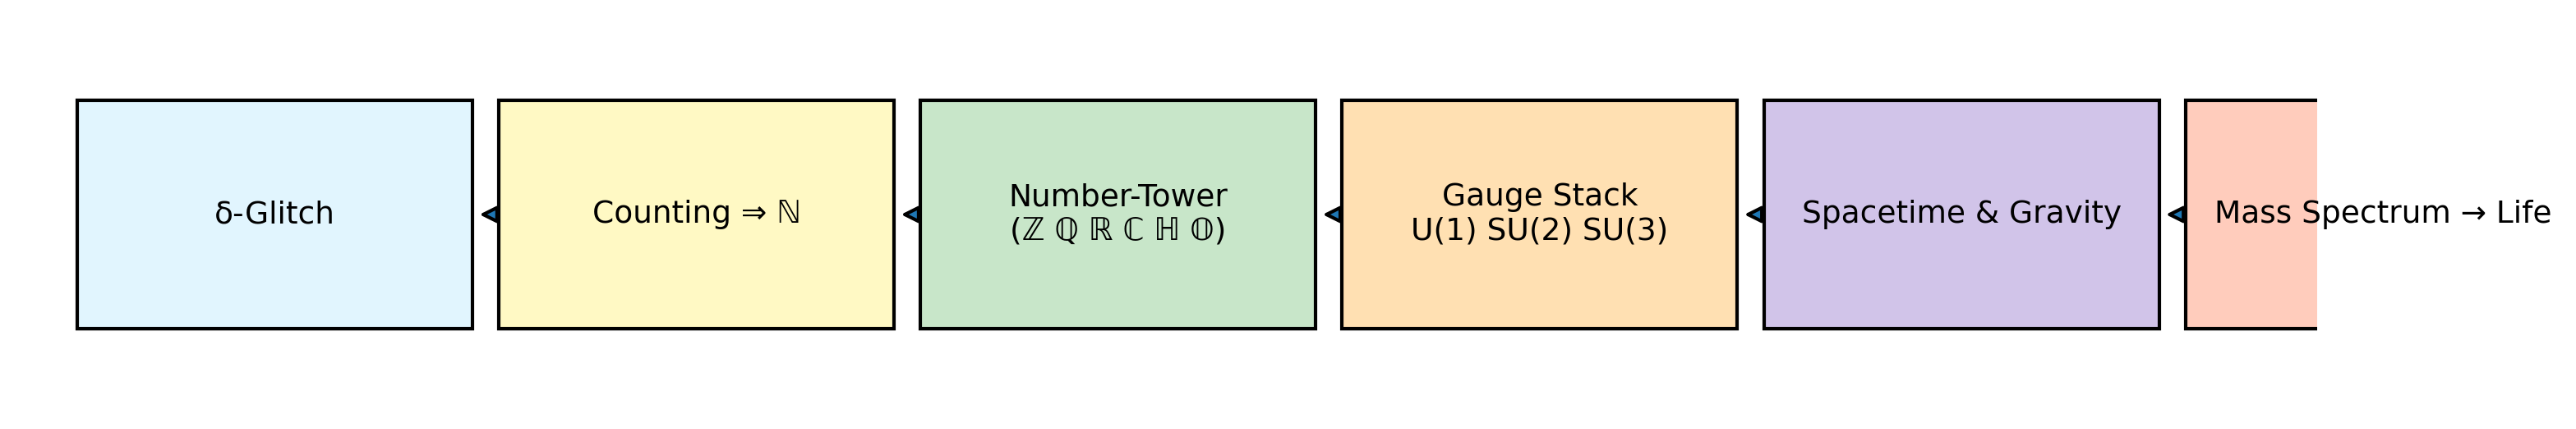
\includegraphics[width=\linewidth]{figs/axiom_flow.png}
  \caption{Logical flow from the two axioms to the structures developed
           in later sections.  No step introduces an external constant.}
  \label{fig:axiom-flow}
\end{figure}

\subsection{Bridge to subsequent sections}

\begin{itemize}
  \item Section \ref{sec:number} constructs $\mathbb C$, $\mathbb H$,
        and $\mathbb O$ purely from ledger counting.
  \item Section \ref{sec:born} proves Born's rule as a weight identity.
  \item Section \ref{sec:gauge} shows how $U(1)\!\times SU(2)\!\times SU(3)$
        gauge symmetry is forced by tag-axis permutations.
\end{itemize}

\clearpage
